\chapter{Introdução}
O ser humano busca cada vez mais produtos que facilitem e tornem tarefas 
diárias mais eficientes. Essa busca gerou ao longo da história inovações e 
aprimoramento de produtos por meio de automações. Historicamente, a automação 
iniciou-se na revolução industrial do século XIX, porém na forma residencial, 
ela surgiu apenas na década de 70, quando foram lançados nos EUA os primeiros 
módulos inteligentes que utilizavam a rede elétrica como canal de comunicação 
entre os diversos dispositivos de automação \cite{bortoluzzi2013}. A partir deste início 
houve um aumento do desenvolvimento de dispositivos dedicados (embarcados) por 
meio da utilização de microprocessadores e microcontroladores. De acordo com 
\citeonline{osorio2010}, o mercado de automação residencial dos Estados Unidos 
movimentou, até 2008, aproximadamente U\$\$ 10,5 bilhões. Além da praticidade 
e conforto, a segurança e eficiência também são fatores importantes para a 
escolha dos produtos residenciais. Dentre algumas das automações residenciais 
modernas destacam-se os aspiradores de pó, que são capazes de realizar a 
aspiração dos resíduos de forma rápida de ambientes sem a dispersão dos 
resíduos. Tendo em vista a necessidade de aspiração em piscinas e a crescente 
onda de automação residencial, observou-se a oportunidade de produzir um 
equipamento para realizar tal tarefa automática de piscinas \cite{kanno2014}.

\section{Contextualização}
O Brasil é o segundo colocado no ranking mundial de países com maior número de 
piscinas, com 1,8 milhão de unidades instaladas (sendo 80\% particulares), 
atrás apenas dos Estados Unidos. O país fatura anualmente cerca de R\$ 4,2 
bilhões com a construção e manutenção de piscinas \cite{portalfatorbrasil2013}. Desta 
forma, atividades relacionadas ao uso da piscina estão cada vez mais 
requisitadas, entre elas a limpeza. A limpeza do fundo da piscina é um processo
que demanda tempo e esforço físico na sua realização . Uma pesquisa realizada 
em  março de 2014 no Estado de São Paulo apontou que o valor médio mensal da 
mão de obra para limpeza de piscinas de até 60 métros cúbicos, com equipamento exceto 
produtos para limpeza e manutenção,  foi de R\$ 303,00. Um valor que se torna 
cada vez mais significativo se imaginarmos piscinas maiores \cite{datafolha2014}. 
Com isso, várias empresas vêm investindo no desenvolvimento de robôs que possam
realizar aspiração de piscinas.No Brasil existem basicamente 3 tipos de 
produtos que realizam a tarefa de limpeza: aspiradores manuais que são os mais 
comuns no mercado, aspiradores robóticos, totalmente automatizados porém com 
alto custo, e aspiradores autônomos porém pouco eficazes \cite{miura2006}.

\section{Justificativa}
Considerando o alto custo de aquisição de equipamentos eficientes, a grande 
demanda por serviços de higienização de piscinas, e o fato de que no Brasil não
há empresas que desenvolvam este produto (há apenas revendedoras), propõe-se o 
desenvolvimento de um produto concorrente. Um robô  que possa realizar a tarefa
de aspiração de  modo satisfatório e com um valor de mercado mais acessível. O 
\textit{Clean Pool Robot} permitirá a aplicação do conceito de automação a 
ambientes residenciais e a redução dos gastos com a contratação de um serviço 
terceirizado. O robô ainda auxilia na privacidade, pois evita o acesso de 
pessoas estranhas à residências ou condomínios. 

\section{Objetivos}
Esse trabalho visa alcançar os objetivos, geral e específicos, apresentados a 
seguir:

\subsection{Objetivo Geral}
O projeto tem por finalidade o desenvolvimento de um robô que realiza a limpeza
do fundo de piscinas.

\subsection{Objetivos Específicos}
Para alcançar o objetivo proposto o projeto irá produzir um protótipo para:
\begin{itemize}
  \item Realizar aspiração automática dos resíduos decantados por meio da sucção e filtragem;
  \item Submergir de forma independente;
  \item Movimentar-se ao longo do fundo da piscina.
 
\end{itemize}

\section{Análise dos Concorrentes}
Um dos primeiros aparelhos utilizados na higienização de piscinas é o Limpa 
Piscina Automático. Este aparelho utiliza o sistema de filtragem da piscina 
como fonte de energia. Fácil de instalar, é necessário apenas ligá-lo à tomada
de aspiração, sem que seja necessário a instalação de quaisquer componentes. 
A potência da bomba da piscina permite que o aparelho se desloque 
automaticamente, de forma a aspirar os resíduos, que ficam retidos no filtro 
da bomba.


\begin{figure}[h]
    \centering
    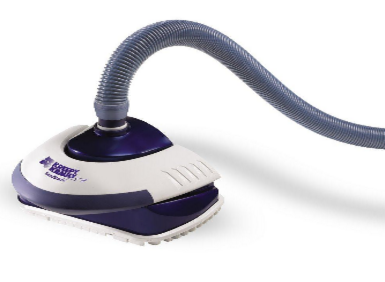
\includegraphics[width=0.5\textwidth]{figures/limpa_piscina_auto.png}
    \caption{Demonstrativo do percurso de limpeza do robô.}
    \label{fig:schema-way-robot}
  \end{figure}

O surgimento do robô limpador de piscina foi uma evolução natural do aspirador 
automático. Este tipo de equipamento é independente do filtro e da bomba da 
piscina, e é alimentado por uma fonte elétrica distinta. Geralmente tem dois 
motores: um associado à sucção da água, fazendo-a passar por um filtro e 
expelindo-a a uma velocidade superior de volta para a piscina, e um motor 
responsável pela locomoção. As cerdas realizam a escovação do fundo da piscina 
e um sistema de controle é responsável por todas as ações relacionadas à 
mudança de direção, detecção de obstáculos, limites e possíveis problemas entre
outras funções. As principais vantagens na utilização do robô são:

\begin{itemize}
  \item retirar detritos que não foram alcançados pelo aspirador;
  \item absorver os detritos flutuantes da água;
  \item mover a água ao passo que limpa as superficies, melhorando a sua circulação.
\end{itemize}
 
Apesar da grande variedade de marcas e modelos, geralmente esses robôs realizam
a mesma função. O peso do aparelho varia de 8 até 25 quilos e  custa no mercado
entre  R\$ 2.000,00 e  R\$ 16.000,00. Há diferenças de especificação a serem 
consideradas na compra, como por exemplo, ciclo de limpeza e taxa de filtragem. 
O ciclo de limpeza determina o intervalo de tempo em que trabalha-se antes de se desligar automaticamente e a taxa de filtragem é determinada pela quantidade de água filtrada em uma 
hora, que é expressa em litros por hora (LPH).

Alguns dos concorrentes pesquisados são descritos na tabela abaixo.

\begin{table}[h]
    \begin{center}
    \begin{tabular}{ c  p{6cm}  }
      \toprule
      Modelo & Especificações \\ 
      \cmidrule(r){1-1}\cmidrule(l){2-2}
      \raisebox{-\totalheight}{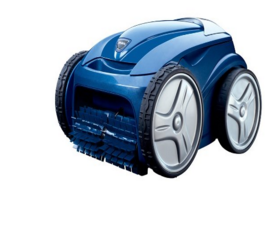
\includegraphics[width=0.3\textwidth]{figures/polaris_sport.png}}
      &
      \textbf{Polaris 9300 \textit{Sport}}
      \begin{itemize}[topsep=0pt]
        \item Duração do ciclo: 2,5 horas;
        \item Peso: 19 kg;
        \item Taxa de filtração: 9 m\textsuperscript{3} LPH;
        \item Preço: R\$ 5.900,00.
      \end{itemize} \\
      Recomendado para piscinas com \\
      comprimento inferior a 12 m. \\
      Possui capacidade pequena de armazenamento. \\
      \\ \bottomrule
    \end{tabular}
     
    \begin{tabular}{ c  p{6cm}  }
      \raisebox{-\totalheight}{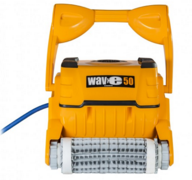
\includegraphics[width=0.2\textwidth]{figures/wave-pentair.png}}
      &
      \textbf{\textit{Wave} 50 - Pentair Sibrape}
      \begin{itemize}[topsep=0pt]
        \item Duração do ciclo: 4 horas;
        \item Peso: 11 kg;
        \item Taxa de filtração: 17 m\textsuperscript{3} LPH;
        \item Preço: R\$ 16.000,00.
      \end{itemize} \\
      Recomendado para piscinas com comprimento \\
      inferior a 20 m. Possui \textit{software} que \\
      permite maximizar cobertura da área.
      \\ \bottomrule
    \end{tabular}
    
    \begin{tabular}{ c  p{6cm}  }
      \raisebox{-\totalheight}{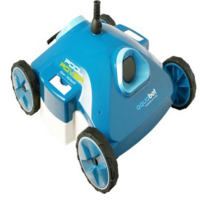
\includegraphics[width=0.2\textwidth]{figures/aquabot-pool.png}}
      &
      \textbf{\textit{Aquabot Pool Rover} S2-40}
      \begin{itemize}[topsep=0pt]
        \item Duração do ciclo: 1 horas;
        \item Peso: 11 kg;
        \item Taxa de filtração: 18 m\textsuperscript{3} LPH;
        \item Preço: R\$ 2.000,00.
      \end{itemize} \\
      Recomendado para piscinas com \\
      comprimento inferior a 10 m. \\
      Adapta-se a diversas piscinas. \\
      \\ \bottomrule
    \end{tabular}
    \caption{Análise de Concorrentes}
    \label{tbl:competitors-analysis}
  \end{center}
\end{table}

\subsection{Visita Técnica}
Para o melhor desenvolvimento do produto e para identificar os possíveis 
concorrentes, foi realizado uma vista técnica na empresa \textit{Aqua Piscina}, na 
sexta-feira 01/04/2016, a uma revendedora de robôs especializados na limpeza de
piscina. Dentre os robôs, foi analisado o que mais se assemelhava com o que 
será desenvolvido por esse trabalho, o \textit{Robot XT5}, conforme ilustrado na 
Figura \ref{fig:robo_visited} abaixo:

\begin{figure}[!htp]
   \centering
    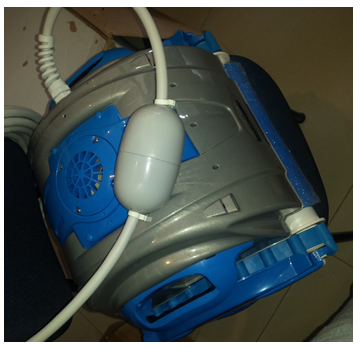
\includegraphics[width=0.35\textwidth]{figures/robo_visited.jpg}
    \caption{Robô visitado}
    \label{fig:robo_visited}
\end{figure}

Durante a visita foi possível analisar como é realizado o processo de sucção e 
filtragem da água e foi observada a disposição dos componentes para tornar o 
aparelho mais eficiente. No sistema de filtragem foi observado a utilização de 
filtro de pano. As escovas que fazem a limpeza assim como o sistema de 
locomoção que é feito por motor elétrico e um sistema de esteira, além do 
sistema de vedação do circuito observados no produto.

\begin{figure}[!h]
   \centering
    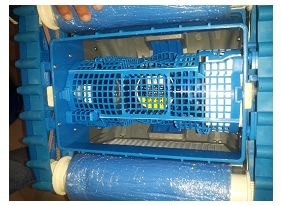
\includegraphics[width=0.4\textwidth]{figures/bottom_view_robot.jpg}
    \caption{Visão inferior do \textit{Robot XT5}}
    \label{fig:bottow_view_robot}
\end{figure}

\begin{figure}[!h]
   \centering
    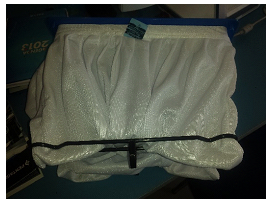
\includegraphics[width=0.6\textwidth]{figures/robot_filter.jpg}
    \caption{Filtro utilizado no \textit{Robot XT5}}
    \label{fig:robot_filter}
\end{figure}

Assim, foi possível analisar todo o sistema do Robot, que vai desde área de 
vedação até a movimentação prática do mesmo. Importante ressaltar que o robô 
analisado apresentou setores muito interessantes, no que se refere ao formato 
e localização dos componentes, os quais poderão ser utilizados de forma 
semelhante no Clean Pool.

